% chktex-file 44
% chktex-file 18
% chktex-file 8
\documentclass{article}
\usepackage{amssymb}
\usepackage{float}
\usepackage{caption}
\usepackage{amsfonts}
\usepackage{amsmath}
\usepackage{cancel}
\usepackage{graphicx}
\graphicspath{ {./assets/} }
\author{Enlai Li}
\title{MATH240 -- Lecture 4}
\date{January 14, 2023}
\begin{document}
\maketitle
\section{Logic continued}
\subsection{Negating a sentence}
Ex:
\begin{itemize}
    \item [p =] you can access the internet on campus \underline{only if} you are a student \underline{or} an employee
    \item [I =] you can access the internet on campus
    \item [S =] you are a student
    \item [E =] you are an employee
\end{itemize}
\[
    p = I \Rightarrow (S \lor E)
\]

Let's find a sentence for $\overline{p}$
\begin{align*}
    \lnot p
     & = \lnot (I \Rightarrow (S \lor E))
    \\ & = \lnot (\lnot I \lor (S \lor E)) \text{ (Def of $\Rightarrow $)}
    \\ & = \lnot \lnot I \land \lnot(S \lor E) \text{ (De Morgan)}
    \\ & =  I \land (\lnot S \land \lnot E) \text{ (De Morgan + Double negation)}
\end{align*}

$ \lnot p =$ You can access the internet on camput and you are not a student and you are not an employee

\subsection{Four types of logical formulas}
A logical formula is:
\begin{itemize}
    \item \underline{satisfiable} if its truth table contains at least one T
    \item a \underline{contradiction} if not satisfiable (always false)
    \item \underline{falsifiable} if its truth table contains at least one F
    \item a \underline{tautology} if not falsifiable (always true)
\end{itemize}
\clearpage

ex1: $p \land \lnot p$: contradiction
\marginpar[]{\raggedright{} contradictions are always falsifiable}
\begin{table}[h]
    \begin{center}
        \begin{tabular}{c|c|c}
            p & $\lnot p$ & $p \land \lnot p$ \\
            \hline
            T & F         & F                 \\
            F & T         & F
        \end{tabular}
    \end{center}
\end{table}

ex2: $p \lor \lnot p$: tautology
\marginpar[]{\raggedright{} tautology are always satisfiable}
\begin{table}[h!]
    \begin{center}
        \begin{tabular}{|c|c|c|}
            \hline
            p & $\lnot p$ & $p \lor \lnot p$ \\
            \hline\hline
            T & F         & T                \\
            F & T         & T                \\
            \hline
        \end{tabular}
    \end{center}
\end{table}

ex3: $p \iff q$: satisfiable and falsifiable
\marginpar[]{\raggedright{} At least one T and one F}
\begin{table}[h!]
    \begin{center}
        \begin{tabular}{|c|c|c|}
            \hline
            p & q & $p \iff q$ \\
            \hline\hline
            T & T & T          \\
            T & F & F          \\
            F & T & T          \\
            F & F & T          \\
            \hline
        \end{tabular}
    \end{center}
\end{table}

\subsection{constant logical formulas}
Formula A is a tautology iff A = 1, and a contradiction iff A = 0
\begin{itemize}
    \item [1:] formula always true
    \item [0:] formula always false
\end{itemize}
ex: show that the following is a tautology
\begin{align*}
    ((p \Rightarrow  q) \land p) \Rightarrow q
    \\ & \equiv ((\lnot p \lor  q) \land p) \Rightarrow q \text{ (Def of $p \Rightarrow  q$)}
    \\ & \equiv \lnot ((\lnot p \lor  q) \land p) \lor q \text{ (Def of $p \Rightarrow  q$)}
    \\ & \equiv (\lnot(\lnot p \lor  q) \lor \lnot p) \lor q \text{ (De Morgan)}
    \\ & \equiv ((p \land \lnot q) \lor \lnot p) \lor q \text{ (De Morgan)}
    \\ & \equiv (p \land \lnot q) \lor (\lnot p \lor q) \text{ (Associative)}
    \\ & \equiv \lnot(\lnot p \lor q) \lor (\lnot p \lor q) \text{ (De Morgan)}
    \\ & \equiv 1 \text{ (Complement)}
\end{align*}

Tautologies can be used for logical reasoning (as inference rules)

\subsection{satisfiability (the SAT problem)}
Given a logical formula, find if it's satisfiable or not. This general problem is much more difficult than it looks. We could always compute the truth table to find out, but with n propositional variable, the table would have $2 ^{n}$ rows! There are softwares called "sat solvers" specialized in solving this problem efficiently (in some cases), but none of them defeats the exponential completely, and it is believed that no such program is possible (this is called the $P \neq NP$ conjecture, 1 million \$ prize attached!)

SAT encodes a lot of practical problem in CS. Ex: Sudoku

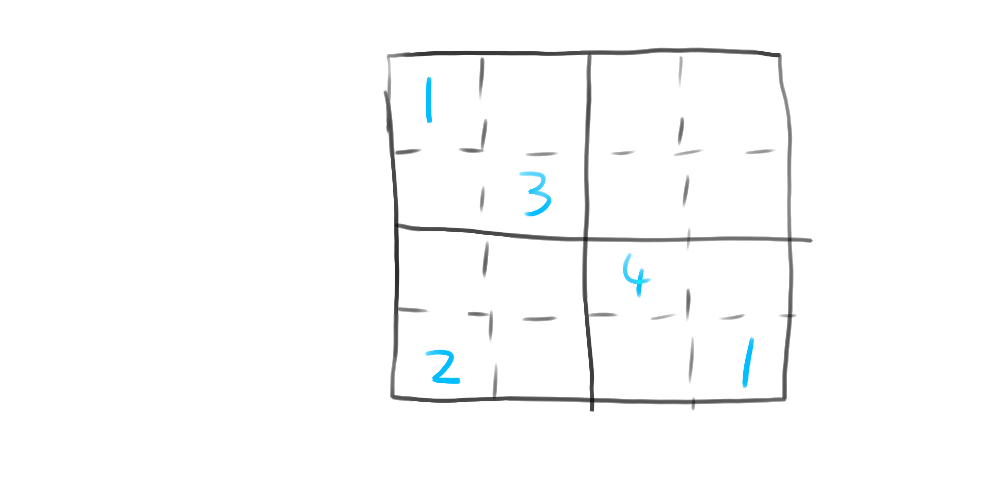
\includegraphics{l4_1}

Fill the grid with numbers \{1,2,3,4\} such that
\begin{enumerate}
    \item Each row contains all 4 numbers
    \item Each column contains all 4 numbers
    \item Each 2x2 contains all 4 numbers
\end{enumerate}
We can solve this using a SAT solver. Variables:
\marginpar[]{\raggedright{} There are 4x4x4 = 64 variables}
\[
    p _{i,j,n} = \text{ "The cell in row i, column j, has value n" }
\]

Then the three conditions translate into formulas:
\begin{enumerate}
    \item $p _{i1n} \lor p _{i2n} \lor p _{i3n} \lor p _{i4n} $ for all i an n in \{1,2,3,4\}
    \item [2.] and 3. : similar
          \\ add some formulas for consistency
    \item [4.] No cell contains two different numbers: \[
              p _{ijn} \Rightarrow \lnot p _{ijk} \text{, for all } i,j,n,k, \text{, where } n \ne k
          \]
    \item [5.] initial conditions: \[
              p _{111} \lor p _{223} \lor p _{334} \lor p _{441} \lor p _{412}
          \]
\end{enumerate}
The conjunction of all the above formulas form a big formula, but a solution which satisfies it is a solution to the sudoku problem
\end{document}